\documentclass{standalone}
\usepackage{tikz}
\usepackage{ctex,siunitx}
\setCJKmainfont{Noto Serif CJK SC}
\usepackage{tkz-euclide}
\usepackage{amsmath}
\usepackage{wasysym}
\usetikzlibrary{patterns, calc}
\usetikzlibrary {decorations.pathmorphing, decorations.pathreplacing, decorations.shapes,}
\begin{document}
\small
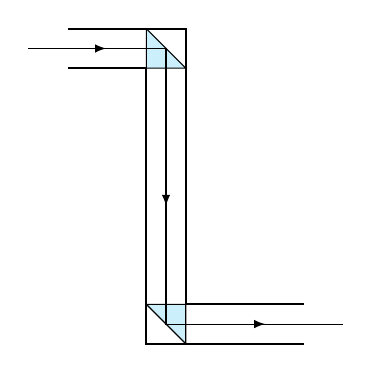
\begin{tikzpicture}[>=latex,scale=1.0]
  \draw [thick](2,0)--(0,0)--(0,3.5)--(-1,3.5);  
  \draw [thick](2,0.5)--(.5,0.5)--(.5,4)--(-1,4);
  \draw [fill=cyan!20](0,0.5)--(.5,.5)--(.5,0)--(0,0.5);
  \draw [fill=cyan!20](0,4)--(0,3.5)--(.5,3.5)--(0,4);
  \draw(-1.5,3.75)--(.25,3.75)--(0.25,.25)--(2.5,.25);
  \draw [postaction ={decorate},decoration={markings,mark={between positions 0.1 and 0.9 step 0.4 with {\arrow{>}}}}](-1.2,3.75)--(.25,3.75)--(0.25,.25)--(2.2,.25);
\end{tikzpicture}
\end{document}